\begin{name}
	{\tenchude}
	{TOÁN 10}
	{LỚP TOÁN THẦY PHÁT}
	{Đừng bao giờ chấp nhận gục ngã trước cuộc sống khó khăn}
\end{name}
\Opensolutionfile{ansbook}[ans/ansbookDe3]
\TN
\Opensolutionfile{ans}[ans/ansDe3-TN1]
\begin{ex}%[TEXHOA-CK2-DOT2-FORM2025-Trần Xuân Hòa]%[0D8N1-2]
Tâm đi từ nhà của mình đến nhà Huyền, cùng Huyền đi đến nhà Linh chơi. Biết từ nhà Tâm đến nhà Huyền có $5$ con đường đi. Từ nhà Huyền đến nhà Linh có $7$ con đường đi. Hỏi có bao nhiêu cách để Tâm đi đến nhà Linh mà phải đi qua nhà Huyền?
\choice
{$12$}
{\True $35$}
{$20$}
{$25$}
\loigiai{
\begin{itemize}
\item Từ nhà Tâm đến nhà Huyền có $5$ cách.
\item Từ nhà Huyền đến nhà Linh có $7$ cách.
\end{itemize}
Theo quy tắc nhân, ta có $5\cdot 7=35$ cách.}
\end{ex}

\begin{ex}%[0D8N2-2]%[Dự án đề kiểm tra Toán 10 Cuối Kì 2 NH23-24- Mui Doan]%[Sở GD Bắc Giang]
Số cách xếp $4$ bạn học sinh $A, B, C, D$ vào $4$ chiếc ghế ngồi theo hàng ngang (mỗi người ngồi một ghế) là
\choice
{$16$}
{$8$}
{$4$}
{\True $24$}
\loigiai{
Mỗi cách xếp là một hoán vị của $4$ phần tử. Số cách xếp là $P_4=4!=24$ cách.
}
\end{ex}

\begin{ex}%[HSA-de10-2526,Lương Pho]%[0D8N3-1]
Trong khai triển nhị thức Newton của $(a+b)^5$ có bao nhiêu số hạng?
\choice
{\True $6$}
{$5$}
{$3$}
{$4$}
\loigiai{
Trong khai triển nhị thức Newton của $(a+b)^n$ có $n+1$ số hạng.\\
Vậy khai triển nhị thức Newton của $(a+b)^5$ có $5+1=6$ số hạng.
}
\end{ex}

\begin{ex}%[10-11-GK2-2425]%[Đỗ Minh Phúc]%[0D6H1-1]
	Cho giá trị gần đúng của $\dfrac{5}{12}$ là $0{,}417$. Sai số tuyệt đối của số $0{,}417$ gần với đáp án nào nhất.
	\choice
	{$0{,}003$}
	{\True $0{,}0003$}
	{$0{,}00003$}
	{$-0{,}0003$}
	\loigiai{
	Sai số tuyệt đối là $\Delta_a=\left|\dfrac{5}{12}-0{,}417\right|\approx 0{,}0003$.
	}
\end{ex}

\begin{ex}%[H]%[BG10-3in1, Phạm Ngọc Trung]%[0D6H4-2]
	\immini{
		Biểu đồ đoạn thẳng ở hình bên biểu diễn giá vàng bán ra trong bảy ngày đầu tiên của tháng $6$ năm $2021$. Tìm khoảng tứ phân vị của mẫu số liệu.
		\choice[1]
		{$29$}
		{\True $30$}
		{$31$}
		{$32$}
	}
	{\begin{tikzpicture}[scale=0.8, font=\footnotesize, line join=round, line cap=round, >=stealth]
			\draw[->,>=stealth,line width=1.5] (0,0)--(0,6); \draw[->,>=stealth,line width=1.5] (0,0)--(8.5,0);
			\path
			(-0.6,0) node {$5 710$}
			(-0.6,1.1) node {$5 722$}
			(-0.6,1.5) node {$5 727$}
			(-0.6,2.5) node {$5737$}
			(-0.6,3.5) node {$5747$}
			(-0.6,4.5) node {$5757$}
			(-0.6,5.5) node {$5767$}
			(0,6.4) node {Giá vàng (nghìn đồng/chỉ)}

			(1,-0.5) node {$1/6$}
			(2,-0.5) node {$2/6$}
			(3,-0.5) node {$3/6$}
			(4,-0.5) node {$4/6$}
			(5,-0.5) node {$5/6$}
			(6,-0.5) node {$6/6$}
			(7,-0.5) node {$7/6$}
			(8.2,-0.5) node {Ngày};

			\draw[line width=1.5] (1,5.5)--(2,4.5)--(3,2.5)--(4,1.5)--(5,3.5)--(6,3.5)--(7,1.2);
			\draw[dashed] (0,5.5)--(1,5.5)--(1,0) (0,4.5)--(2,4.5)--(2,0) (0,2.5)--(3,2.5)--(3,0) (0,1.5)--(4,1.5)--(4,0) (0,3.5)--(5,3.5)--(5,0) (6,3.5)--(6,0) (0,1.2)--(7,1.2)--(7,0);
			\fill[black] (1,5.5) circle (2.5pt);
			\fill[black] (2,4.5)circle (2.5pt);
			\fill[black] (3,2.5)circle (2.5pt);
			\fill[black] (4,1.5)circle (2.5pt);
			\fill[black] (5,3.5)circle (2.5pt);
			\fill[black] (6,3.5)circle (2.5pt);
			\fill[black] (7,1.2) circle (2.5pt);
		\end{tikzpicture}
	}
	\loigiai{
		\begin{itemize}
			\item 	Mẫu số liệu thống kê tốc độ tăng trưởng GDP nhận được
			      \begin{center}
				      \begin{tabular}{|c|c|c|c|c|c|c|c|}
					      \hline
					      Ngày                      & $1/6$  & $2/6$  & $3/6$  & $4/6$  & $5/6$  & $6/6$  & $7/6$  \\
					      \hline
					      Giá vàng (nghìn đồng/chỉ) & $5767$ & $5757$ & $5737$ & $5727$ & $5747$ & $5747$ & $5722$ \\
					      \hline
				      \end{tabular}\\
				      Sắp xếp lại mẫu số liệu ta được \\
				      \begin{tabular}{cccccccc}
					       & $5722$ & $5727$ & $5737$ & $5747$ & $5747$ & $5757$ & $5767$
				      \end{tabular}
			      \end{center}
			\item
			      Ta có $Q_2=5747; \; Q_1=5727; \; Q_3=5757$.\\
			      Vậy khoảng tứ phân vị $\Delta_Q=Q_3-Q_1=5757-5727=30$.
		\end{itemize}
	}
\end{ex}

\begin{ex}%[0D0N1-2]
	Tung một đồng xu và một con xúc xắc, nhận được kết quả là mặt xuất hiện trên đồng xu (sấp hay ngửa) và số chấm xuất hiện trên con xúc xắc. Số kết quả có thể xảy ra là
	\choice
	{$2$}
	{$6$}
	{$8$}
	{\True $12$}
	\loigiai{
		Đồng xu chỉ có hai mặt sấp hay ngửa.\\
		Con xúc xắc số chấm xuất hiện là $1,2,3,4,5,6$.\\
		Số kết quả có thể xảy ra là $2\cdot 6=12$.
	}
\end{ex}

\begin{ex}%[0D0N1-3]
	Gieo một đồng tiền và một con xúc xắc. Số phần tử của không gian mẫu là
	\choice
	{$24$}
	{\True $12$}
	{$6$}
	{$8$}
	\loigiai{
		Mô tả không gian mẫu ta có $\Omega=\{S1; S2; S3; S4; S5;S6;N1;N2;N3;N4;N5;N6\}$.
	}
\end{ex}

\begin{ex} %[0H9N3-1]
	Trong mặt phẳng $O x y$, cho đường thẳng $\Delta$ có phương trình $\dfrac{x-1}{2}=\dfrac{y+1}{-1}$. Vectơ chỉ phương của đường thẳng $\Delta$ là
	\choice
	{\True $\vec{u}(2 ;-1)$}
	{$\vec{u}(1 ; 2)$}
	{$\vec{u}(1 ;-1)$}
	{$\vec{u}(1 ; 1)$}
	\loigiai{
		Từ phương trình đường thẳng $\Delta$ suy ra vectơ chỉ phương của đường thẳng $\Delta$ là $\vec{u}(2 ;-1)$.
	}
\end{ex}

\begin{ex}
	Trong mặt phẳng $Oxy$, khoảng cách từ điểm $A(x_0;y_0)$ đến đường thẳng $\Delta \colon ax+by+c=0$ được tính bằng công thức
	\choice
	{$d=\dfrac{|ax_0+by_0+c|}{\sqrt{a^2+b^2}}$}
	{$d=\dfrac{|ax_0+by_0-c|}{\sqrt{a^2+b^2}}$}
	{\True $d=\dfrac{|ax_0+by_0+c|}{\sqrt{a^2+b^2}}$}
	{$d=\dfrac{|ax_0-by_0+c|}{\sqrt{a^2+b^2}}$}
	\loigiai{
		Ta có công thức tính khoảng cách từ điểm $A(x_0;y_0)$ đến đường thẳng $\Delta \colon ax+by+c=0$ là
		$d=\dfrac{|ax_0+by_0+c|}{\sqrt{a^2+b^2}}.$
	}
\end{ex}

\begin{ex}%[0H9N3-3]
	Cho hai đường thẳng $\Delta_1\colon \sqrt{7}x-2y-3=0$ và $\Delta_2\colon 2x-\sqrt{7}y+3=0$. Vị trí tương đối của $2$ đường thẳng này là
	\choice
	{\True $\Delta_1$ cắt $\Delta_2$ và $\Delta_1 \not \perp \Delta_2$}
	{$\Delta_1$ song song $\Delta_2$}
	{$\Delta_1$ trùng $\Delta_2$}
	{$\Delta_1$ cắt $\Delta_2$ và $\Delta_1 \perp \Delta_2$}
	\loigiai{
		Ta có $\heva{&\Delta_1\colon \sqrt{7}x-2y-3=0\\ &\Delta_2\colon 2x-\sqrt{7}y+3=0}\Leftrightarrow \heva{&x=2+\sqrt{7}\\ &y=2+\sqrt{7}.}$\\
		Vì $\overrightarrow{n}_{\Delta_1}\cdot\overrightarrow{n}_{\Delta_2}=\sqrt{7}\cdot2+(-2)\cdot\left(-\sqrt{7}\right)=4\sqrt{7}\neq0$.\\
		Nên $\Delta_1$ cắt $\Delta_2$ nhưng không vuông góc.
	}
\end{ex}

\begin{ex}%[0H9N5-1]%[Dự án đề kiểm tra Toán Khối 10 CK2 NH23-24-Dot 16- Khắc Thiên]%[THPT Chuyên Hùng Vương - Phú Thọ]
	Trong mặt phẳng $Oxy$, cho đường elip $(E)$ có phương trình  $\dfrac{x^2}{36}+\dfrac{y^2}{9}=1$. Tổng khoảng cách từ mỗi điểm trên elip tới hai tiêu điểm bằng
	\choice
	{$6$}
	{$3$}
	{$5$}
	{\True $12$}
	\loigiai{
		Ta có phương trình của chính tắc elip  $(E)$ là $\dfrac{x^2}{36}+\dfrac{y^2}{9}=1$.\\
		Suy ra $a=6$.\\
		Khi đó, tổng khoảng cách từ mỗi điểm trên elip tới hai tiêu điểm bằng $2a=12$.
	}
\end{ex}

\begin{ex}%[0H9N5-5]%[Dự án đề kiểm tra Toán Khối 10 CK2 NH23-24-Dot 16- Khắc Thiên]%[THPT Chuyên Hùng Vương - Phú Thọ]
	Phương trình nào sau đây là phương trình chính tắc của hypebol?
	\choice
	{$\dfrac{x^2}{9}+\dfrac{y^2}{4}=1$}
	{$\dfrac{x^2}{4}-\dfrac{y^2}{9}=-1$}
	{\True $\dfrac{x^2}{4}-\dfrac{y^2}{9}=1$}
	{$\dfrac{x^2}{9}+\dfrac{y^2}{9}=1$}
	\loigiai{
		Phương trình chính tắc của hypebol có dạng $\dfrac{x^2}{a^2}-\dfrac{y^2}{b^2}=1$ (với $a>0$, $b>0$) nên $\dfrac{x^2}{4}-\dfrac{y^2}{9}=1$ là  phương trình chính tắc của hypebol.
	}
\end{ex}
\Closesolutionfile{ans}

\TNTF
\Opensolutionfile{ans}[ans/ansDe3-TN2]
\begin{ex}%[0D6H4-2]%[Dự án đề kiểm tra Toán 11 GHKII NH23-24- Hieu Hieu Minh Minh]%[THPT Toàn Thắng- Hải Phòng]
	Điều tra về chiều cao (đơn vị: $\mathrm{cm}$ ) của $12$ học sinh tổ $1$ lớp $10 \mathrm{C}$ thu được bảng số liệu sau: \[\begin{array}{llllllllllll}
			154 & 150 & 152 & 160 & 165 & 168 & 154 & 170 & 163 & 172 & 152 & 160
		\end{array}\]
	Khi đó:
	\choiceTF
	{Mẫu số liệu có khoảng tứ phân vị là $6 \mathrm{cm}$}
	{\True Độ chênh lệch chiều cao tối đa của các học sinh là $22 \mathrm{cm}$}
	{\True Quy tròn phương sai của mẫu số liệu với độ chính xác $d=0,5$ là $54$}
	{\True Sai số tương đối của số quy tròn phương sai trên xấp xỉ $0,9\%$}
	\loigiai{
		\begin{itemchoice}
			\itemch Sai.
			\begin{itemize}
				\item Nửa số liệu bên trái là $150$; $152$; $152$; $154$; $154$; $160$ gồm  $6$  giá trị nên $Q_1=153$.
				\item  Nửa số liệu bên phải là $160$; $163$; $165$; $168$; $170$; $172$ gồm  $6$  giá trị nên $Q_3=166{,}5$.
			\end{itemize}
			Do đó khoảng tứ phân vị của mẫu số liệu bằng $\Delta_Q=Q_3-Q_1=166{,}5-160=6{,}5$.
			\itemch Đúng. Chiều cao nhỏ nhất là $150 \mathrm{cm}$ và chiều cao lớn nhất là $172\mathrm{cm}$ nên độ chênh lệch chiều cao tối đa của các học sinh là $22\mathrm{cm}$.
			\itemch Sai.\\
			Sử dụng máy tính bỏ túi ta được phương sai mẫu là $53,5$.\\
			Vậy quy tròn phương sai của mẫu số liệu với độ chính xác $d=0,5$ là $54$.
			\itemch Sai.\\
			Sai số tương đối của số quy tròn phương sai là
			\[\delta=\dfrac{54-53,5}{54}\approx 0,009\approx 0,9\%.\]
		\end{itemchoice}
	}
\end{ex}

\begin{ex}%[0H9H3-2]%[0H9H3-3]
	Trong mặt phẳng tọa độ $Oxy$, cho đường thẳng $d_1\colon x-2y+3=0$; $d_2\colon 3x-y-1=0$ và điểm $A(2;1)$.
	\choiceTF
	{Đường thẳng đi qua $A$ và song song với $d_1$ có phương trình $2x+y-5=0$}
	{\True Hai đường thẳng $d_1$ và $d_2$ cắt nhau tại điểm $M(1;2)$}
	{Phương trình đường tròn tâm $A$ đi qua $M$ là $(x-2)^2+(y-1)^2=5$}
	{Tiếp tuyến của đường tròn $(A)$ tại $M$ có phương trình $x-2y+1=0$}
	\loigiai{
		\begin{itemchoice}
			\itemch {\bf Sai}.\\
			Gọi $\Delta_1$ là đường thẳng song song với $d_1$.\\
			Suy ra $\Delta_1$ có phương trình dạng $x-2y+c=0$.\\
			Mặt khác, $\Delta_1$ đi qua $A(2;1)$ suy ra $2-2\cdot 1+c=0\Rightarrow c=0$.\\
			Vậy, đường thẳng đi qua $A$ và song song với $d_1$ có phương trình $x-2y=0$.
			\itemch {\bf Đúng}.\\
			Giao điểm của $d_1$ và $d_2$ là nghiệm của hệ phương trình $\heva{&x-2y+3=0\\&3x-y-1=0.}$\\
			Giải hệ ta được $\heva{&x=1\\&y=2.}$\\
			Vậy, hai đường thẳng $d_1$ và $d_2$ cắt nhau tại điểm $M(1;2)$.
			\itemch {\bf Sai}.\\
			Đường tròn $(A)$ có tâm $A(2;1)$ và đi qua $M(1;2)$ nên có bán kính $R=AM=\sqrt{(2-1)^2+(1-2)^2}=\sqrt{2}$.\\
			Vậy, phương trình đường tròn $(A)$ là $(x-2)^2+(y-1)^2=2$.
			\itemch {\bf Sai}.\\
			Ta có phương trình tiếp tuyến của đường tròn $(A)$ tại điểm $M(1;2)$ là
			\[(x-2)(1-2)+(y-1)(2-1)=0\Leftrightarrow (x-2)+y-1=0\Leftrightarrow x+y-3=0.\]
		\end{itemchoice}
	}
\end{ex}
\Closesolutionfile{ans}

\TNSA
\Opensolutionfile{ans}[ans/ansDe3-TN3]
\begin{ex}%[H]giảng 10 New - 4in1, Nguyễn Vân Trường]%[0D8H1-3]
Từ các chữ số $0$, $1$, $2$, $7$, $8$, $9$ tạo được bao nhiêu số chẵn có $5$ chữ số khác nhau?
\shortans{$312$}
\loigiai{
Gọi số chẵn có $5$ chữ số khác nhau thỏa mãn đề bài là $\overline{abcde}$.
\begin{itemize}
\item Nếu $e = 0$ thì $a$ có $5$ cách chọn, $b$ có $4$ cách chọn, $c$ có $3$ cách chọn, $d$ có $2$ cách chọn. Suy ra có tất cả $5\cdot 4\cdot 3\cdot 2= 120$ số.
\item Nếu $e\in\{2;8\}$ thì $a$ có $4$ cách chọn, $b$ có $4$ cách chọn, $c$ có $3$ cách chọn, $d$ có $2$ cách chọn. Suy ra có tất cả $2\cdot 4\cdot 4\cdot 3\cdot 2= 192$ số
\end{itemize}
Vậy số các số có $5$ chữ số thỏa mãn đề bài là $120 + 192 = 312$ số.
}
\end{ex}

\begin{ex}%[24-25 giảng K10 - K11, Phan Quốc Trí]%[0D8V2-4]
Cho $12$ học sinh gồm $3$ học sinh khối $12$, $4$ học sinh khối $11$ và $5$ học sinh khối $10$. Có bao nhiêu cách chọn $6$ học sinh từ $12$ học sinh đó sao cho mỗi khối có ít nhất một người?
\shortans[oly]{805}
\loigiai{
Do số học sinh của mỗi khối đều nhỏ hơn $6$ nên khi chọn $6$ bạn bất kì luôn có ít nhất học sinh của hai khối được chọn, để tính số cách chọn thoả mãn bài ra ta chỉ cần loại số cách chọn chỉ có đúng học sinh của hai khối được chọn.\\
Số cách chọn $6$ học sinh bất kì trong $12$ học sinh là $\mathrm{C}^6_{12}$ cách.\\
Số cách chọn $6$ học sinh bất kì trong $7$ học sinh của hai khối $11$ và $12$ là $\mathrm{C}^6_7$ cách.\\
Số cách chọn $6$ học sinh bất kì trong $9$ học sinh của hai khối $10$ và $11$ là $\mathrm{C}^6_9$ cách.\\
Số cách chọn $6$ học sinh bất kì trong $8$ học sinh của hai khối $10$ và $12$ là $\mathrm{C}^6_8$ cách.\\
Vậy có tất cả $\mathrm{C}^6_{12} - \left( \mathrm{C}^6_7 + \mathrm{C}^6_8 + \mathrm{C}^6_9 \right) = 805$ cách chọn thoả mãn yêu cầu.
}
\end{ex}

\begin{ex}%[0H9V5-0]
\immini
{
Một tòa tháp (hình bên) có mặt cắt là một đường hypebol và có chiều cao $200$ m, chỗ nhỏ nhất ở chính giữa và rộng $50$ m, đỉnh tháp và đáy tháp có độ rộng đều bằng $60$ m. Độ rộng của tòa tháp ở độ cao $150$ m bằng bao nhiêu (kết quả tính theo đơn vị mét và làm tròn đến hàng phần chục)?
}
{
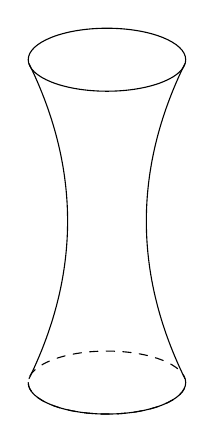
\begin{tikzpicture}[line join = round, line cap = round,>=stealth,scale=1,font=\footnotesize]
%		\draw[->] (-2,0) -- (2,0) node[right] {$x$};
%		\draw[->] (0,-3) -- (0,3.2) node[above] {$y$};
\draw[domain=-2:2,smooth, samples=150] plot ({(0.35*(\x))^(2)+0.5},\x);
\draw[domain=-2:2,smooth, samples=150] plot (-{(0.35*(\x))^(2)-0.5},\x);
\draw (0,2.05) ellipse (1 and 0.4);
\draw[dashed] (0,-2.05) ellipse (1 and 0.4);
\draw (0,-2.05)+(0:1 and 0.4) arc (0:-180:1 and 0.4);
\end{tikzpicture}
}
\shortans{$52{,}7$}
\loigiai{
\immini
{
Gắn hệ trục tọa độ $Oxy$ như hình bên, $1$ đơn vị đo tương ứng $1$ m.\\
Phương trình chính tắc của hypebol $(H)\colon \dfrac{x^2}{a^2}-\dfrac{y^2}{b^2}=1,\ (a > 0, b> 0)$.\\
Theo giả thiết ta có $2a=50\Rightarrow a=25$.\\
Mặt khác $(H)$ đi qua $M(30;100)$ nên ta có $\dfrac{30^2}{25^2}-\dfrac{100^2}{b^2}=1\Rightarrow b^2=\dfrac{250000}{11}\Rightarrow (H)\colon \dfrac{x^2}{625}-\dfrac{y^2}{\dfrac{250000}{11}}=1$.
}
{
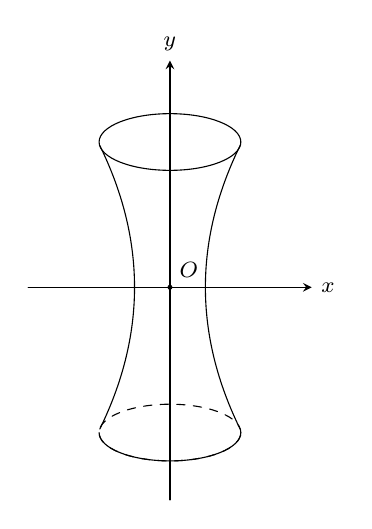
\begin{tikzpicture}[line join = round, line cap = round,>=stealth,scale=0.9,font=\footnotesize]
\draw[->] (-2,0) -- (2,0) node[right] {$x$};
\draw[->] (0,-3) -- (0,3.2) node[above] {$y$};
\draw[domain=-2:2,smooth, samples=150] plot ({(0.35*(\x))^(2)+0.5},\x);
\draw[domain=-2:2,smooth, samples=150] plot (-{(0.35*(\x))^(2)-0.5},\x);
\draw (0,2.05) ellipse (1 and 0.4);
\draw[dashed] (0,-2.05) ellipse (1 and 0.4);
\draw (0,-2.05)+(0:1 and 0.4) arc (0:-180:1 and 0.4);
\fill (0,0)node[above right]{$O$} circle (1pt);
\end{tikzpicture}
}
\noindent Độ rộng của tháp ở độ cao $150$ m ứng với điểm $N(x;50)\in (H)$ nên ta có
\[\dfrac{x^2}{625}-\dfrac{50^2}{\tfrac{250000}{11}}=1\Rightarrow x=\dfrac{5\sqrt{111}}{2}.\]
Suy ra độ rộng của tháp ở độ cao $150$ m là $2x=\dfrac{2\cdot 5\sqrt{111}}{2}=52{,}7\ \mathrm{(m)}$.
}
\end{ex}

\begin{ex}%[0H9V4-2]
	Trong mặt phẳng với hệ tọa độ $Oxy$, cho đường thẳng $d\colon 2x-y-5=0$ và hai điểm $A\left(1;2\right), B\left(4;1\right)$. Tính bán kính đường tròn $(C)$ có tâm thuộc $d$ và đi qua hai điểm $A, B$.
	\shortans{$5$}
	\loigiai{
		\immini{
			Gọi $I$ là tâm của $(C)$. Do $I\in d$ nên $I\left(t;2t-5\right)$.\\
			Hai điểm $A, B$ cùng thuộc $(C)$ nên
			\begin{align*}
				IA=IB & \Leftrightarrow (1-t)^2+\left(7-2t\right)^2=(4-t)^2+\left(6-2t\right)^2 \\
				      & \Leftrightarrow t=1.
			\end{align*}
			Suy ra $I(1;-3)$ và bán kính $R=IA=5$.\\

		}
		{
			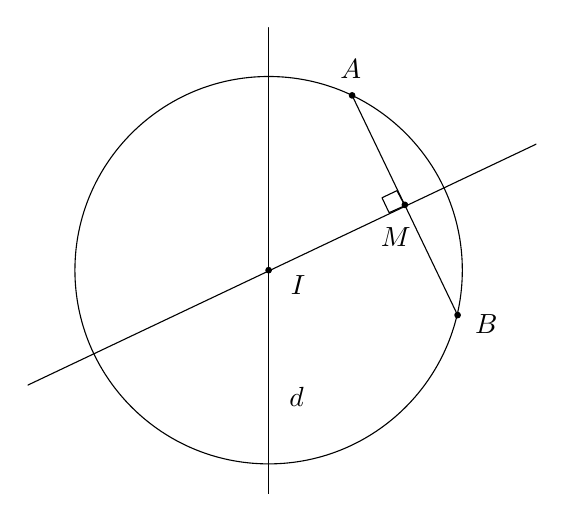
\begin{tikzpicture}[line cap=round,line join=round,>=stealth,x=1.0cm,y=1.0cm]
				\clip(1.24,-1.) rectangle (7.7,4.92);
				\draw (5.93,2.85) -- (5.74,2.76) -- (5.83,2.57) -- (6.03,2.66) -- cycle;
				\draw (4.3,1.84) circle (2.46cm);
				\draw (5.36,4.06)-- (6.7,1.27);
				\draw [domain=1.24:7.7] plot(\x,{(-0.36--0.82*\x)/1.73});
				\draw (4.3,-1.) -- (4.3,4.92);
				\draw (5.6,4.4) node[left] {$A$};
				\draw (6.8,1.4) node[anchor=north west] {$B$};
				\draw (5.6,2.5) node[anchor=north west] {$M$};
				\draw (4.44,0.48) node[anchor=north west] {$d$};
				\draw (4.46,1.9) node[anchor=north west] {$I$};
				\draw [fill=black] (4.3,1.84) circle (1.0pt);
				\draw [fill=black] (5.36,4.06) circle (1.0pt);
				\draw [fill=black] (6.7,1.27) circle (1.0pt);
				\draw [fill=black] (6.03,2.67) circle (1.0pt);
			\end{tikzpicture}
		}
	}
\end{ex}

\Closesolutionfile{ans}

\TL
\begin{ex}
	Tìm số hạng không chứa $x$ trong khai triển nhị thức Newton của $\left(x+\dfrac{1}{x}\right)^4$.
\end{ex}


\begin{ex}%[0H9V4-5]%[Dự án đề kiểm tra Toán 11 GHKI NH23-24- Phan Anh]%[THPT - Tp HCM]
Trong mặt phẳng tọa độ $Oxy$, cho điểm $I(2;-1)$ và đường thẳng $d\colon3x+y+5=0$. Đường tròn $(C)$ có tâm $I$ và đường kính bằng $4\sqrt{5}$. Đường thẳng $\Delta\colon x+by+c=0$, $c>0$ vuông góc với đường thẳng $d$ và cắt $(C)$ tại hai điểm phân biệt $A$, $B$ sao cho tam giác $IAB$ tù và có diện tích bằng $5\sqrt{3}$.
\begin{enumerate}
	\item Viết phương trình đường tròn $(C)$.
	\item Tìm hệ số $b$ và $c$ của đường thẳng $\Delta$.
\end{enumerate}
\loigiai{\immini{Đường tròn $(C)$ có đường kính bằng $4\sqrt{5}$ nên có bán kính là $R=2\sqrt{5}$.\\
Đường thẳng $\Delta$ vuông góc với đường thẳng $d$ nên $\Delta\colon x-3y+c=0$.\\
Tam giác $IAB$ có diện tích là $5\sqrt{3}$ nên
\[S=\dfrac{1}{2}\cdot IA\cdot IB\cdot\sin\widehat{AIB}\Leftrightarrow5\sqrt{3}=\dfrac{R^2\sin\widehat{AIB}}{2}\Leftrightarrow\sin\widehat{AIB}=\dfrac{\sqrt{3}}{2}.\]}
{\begin{tikzpicture}[>=stealth,line join=round,line cap=round,font=\footnotesize,scale=0.3]
\path (0,0) coordinate (I)
($(I)+({5*cos(30)},{5*sin(30)})$) coordinate(A)
($(I)!1!120:(A)$) coordinate(B)
($(A)!0.5!(B)$) coordinate(H)
;
\draw (I)circle(5);
\draw (H)--(I)--(B)--(A)--(I);
\foreach \p / \r in {A/45,I/-90,B/135,H/90}
\fill (\p) circle (1.2pt) node[shift={(\r:3mm)}]{$\p$};
\end{tikzpicture}}
\noindent
Do $\triangle IAB$ tù nên $\widehat{AIB}=120^\circ$, suy ra khoảng cách từ $I$ đến $\Delta$ là $IH=\dfrac{R}{2}=\sqrt{5}$.\\
Từ đó ta có $IH=\mathrm{d}(I,\Delta)=\dfrac{|2+3+c|}{\sqrt{1+9}}=\sqrt{5}\Leftrightarrow\hoac{&c=5\sqrt{2}-5\\&c=-5\sqrt{2}-5.}$\\
Do $c$ dương nên nhận $c=5\sqrt{2}-5\approx2{,}1$.}
\end{ex}

\begin{ex}%[0D0C1-3]%[Phạm Hoàng Điệp]%[Đợt 1 - HSA - Đề 22]
Một con kiến di chuyển trên một bàn cờ từ ô vuông A đến ô vuông B như hình vẽ. Trong một lần di chuyển, con kiến chỉ có thể di chuyển sang ô bên phải hoặc xuống ô phía dưới. Trong bàn cờ có một số ô vuông chứa các vật cản được đánh dấu, con kiến không thể đi vào các ô vuông đó. Hỏi con kiến có bao nhiêu cách đi từ ô vuông $A$ tới ô vuông $B$?
\begin{center}
\begin{tikzpicture}
\matrix (m) [matrix of nodes, nodes={minimum height=1cm, minimum width=1cm, draw, thick, anchor=center, align=center}, nodes in empty cells]
{
$A$&&&&\\
&&&&$\times$\\
&$\times$&&&\\
&&$\times$&&$B$\\
};
\end{tikzpicture}
\end{center}

\loigiai{
Số cách đi tới một ô vuông sẽ bằng tổng số cách đi tới ô vuông ngay trên nó và số cách đi tới ô vuông bên trái nó.\\
Nếu ô vuông đó không thể đi vào, số cách đi vào ô vuông đó sẽ bằng $0$.\\
Qua đó, ta có bảng số cách đi tới từng ô vuông như sau
\begin{longtable}{|m{0.7cm}|m{0.7cm}|m{0.7cm}|m{0.7cm}|m{0.7cm}|}
\hline
$1$ & $1$ & $1$ & $1$ & $1$ \\ \hline
$1$ & $2$ & $3$ & $4$ & $0$ \\ \hline
$1$ & $0$ & $3$ & $7$ & $7$ \\ \hline
$1$ & $1$ & $0$ & $7$ & $14$ \\
\hline
\end{longtable}
Như vậy, có $14$ cách cho con kiến đi tới ô vuông $B$ từ ô vuông $A$.
}
\end{ex}
\Closesolutionfile{ansbook}
